\documentclass{phyasgn}\usepackage{nag}
\phyasgn{classname=Ultrafast Laser and Spectroscopy}
\usepackage[backend=bibtex,bibstyle=gb7714-2015,citestyle=gb7714-2015]{biblatex}
\renewcommand\refname{Reference}
\renewcommand{\figurename}{Fig.}
\newcommand{\figref}[1]{Fig.~\ref{#1}}
\setlength{\bibitemsep}{3bp}
\usepackage{background}
\backgroundsetup{scale=1,angle=0,opacity=1,contents={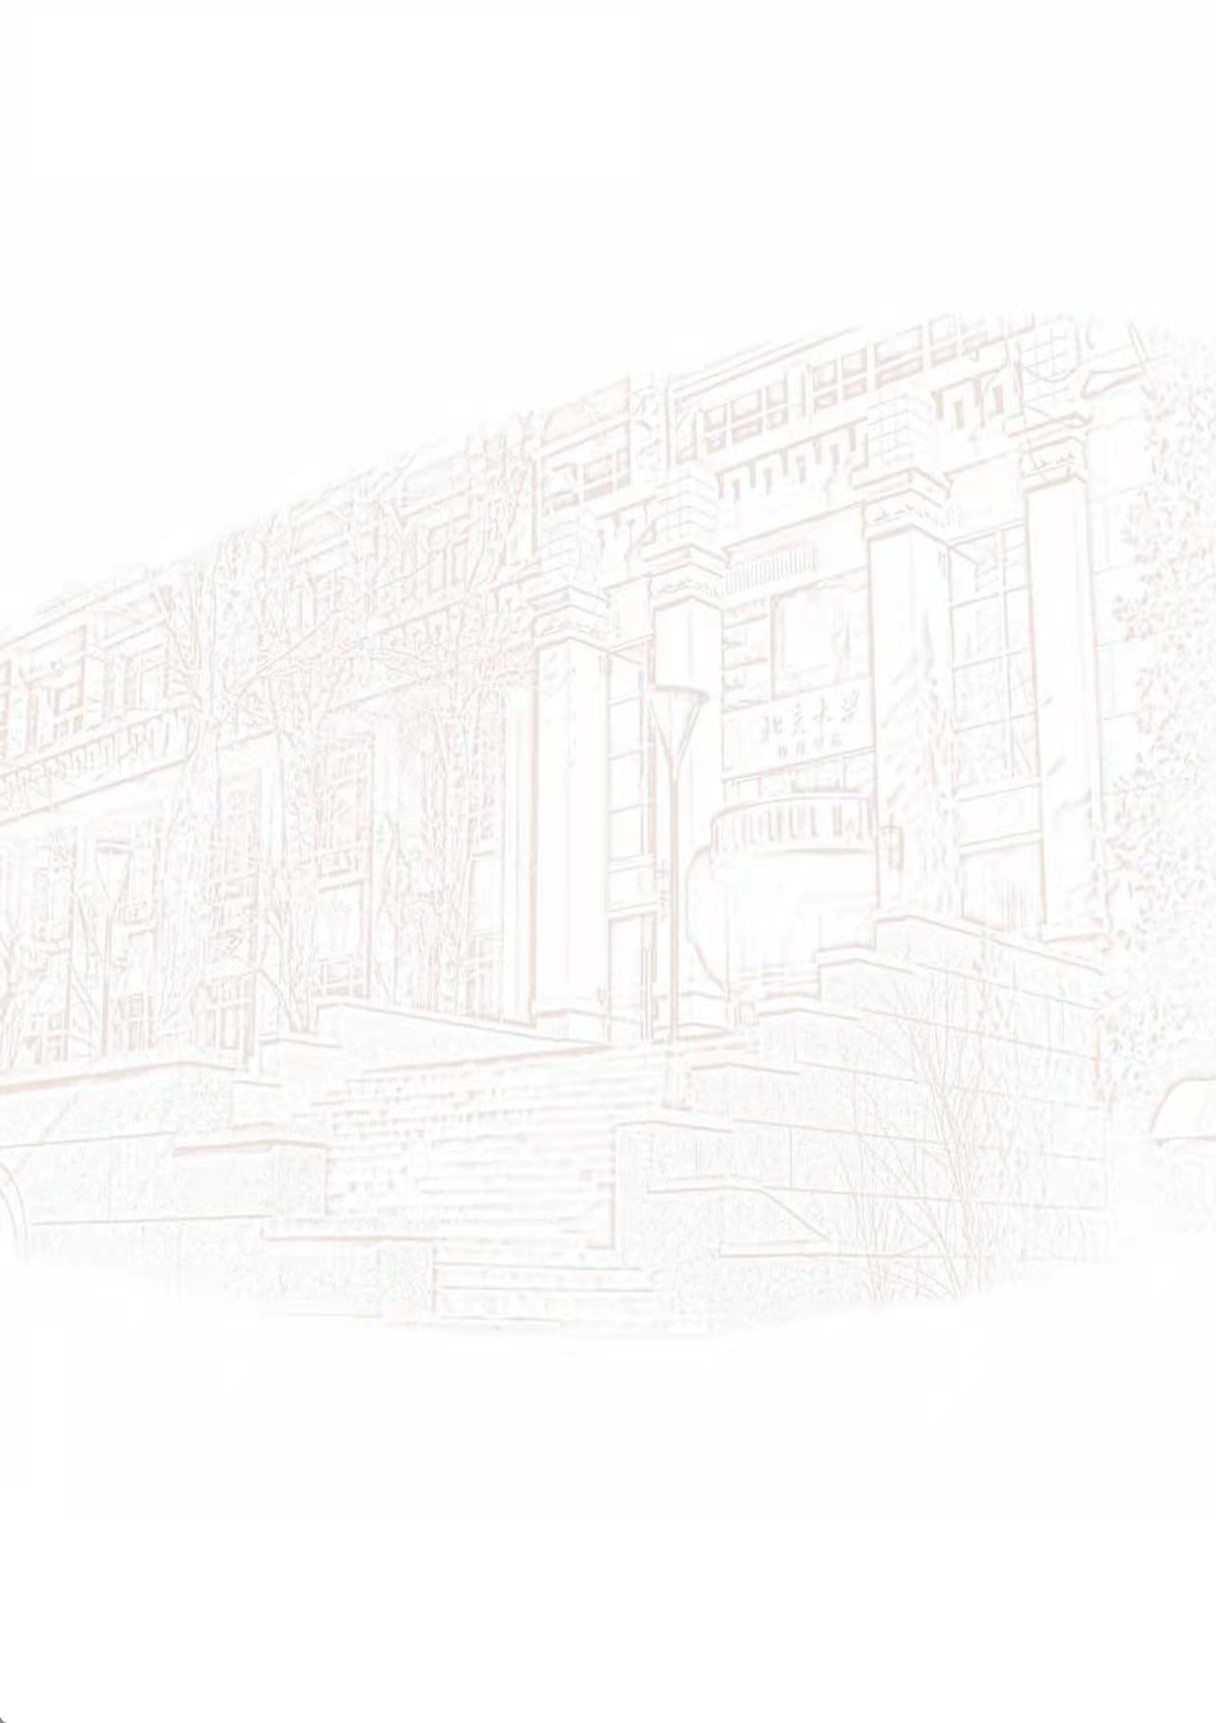
\includegraphics[width=\paperwidth, height=\paperwidth, keepaspectratio]{pic/phy.jpg}}}
\addbibresource{ref.bib}
\renewcommand*{\bibfont}{\zihao{5}\linespread{1.27}\selectfont}
%\usepackage{background}
%\backgroundsetup{scale=1,angle=0,opacity=1,contents={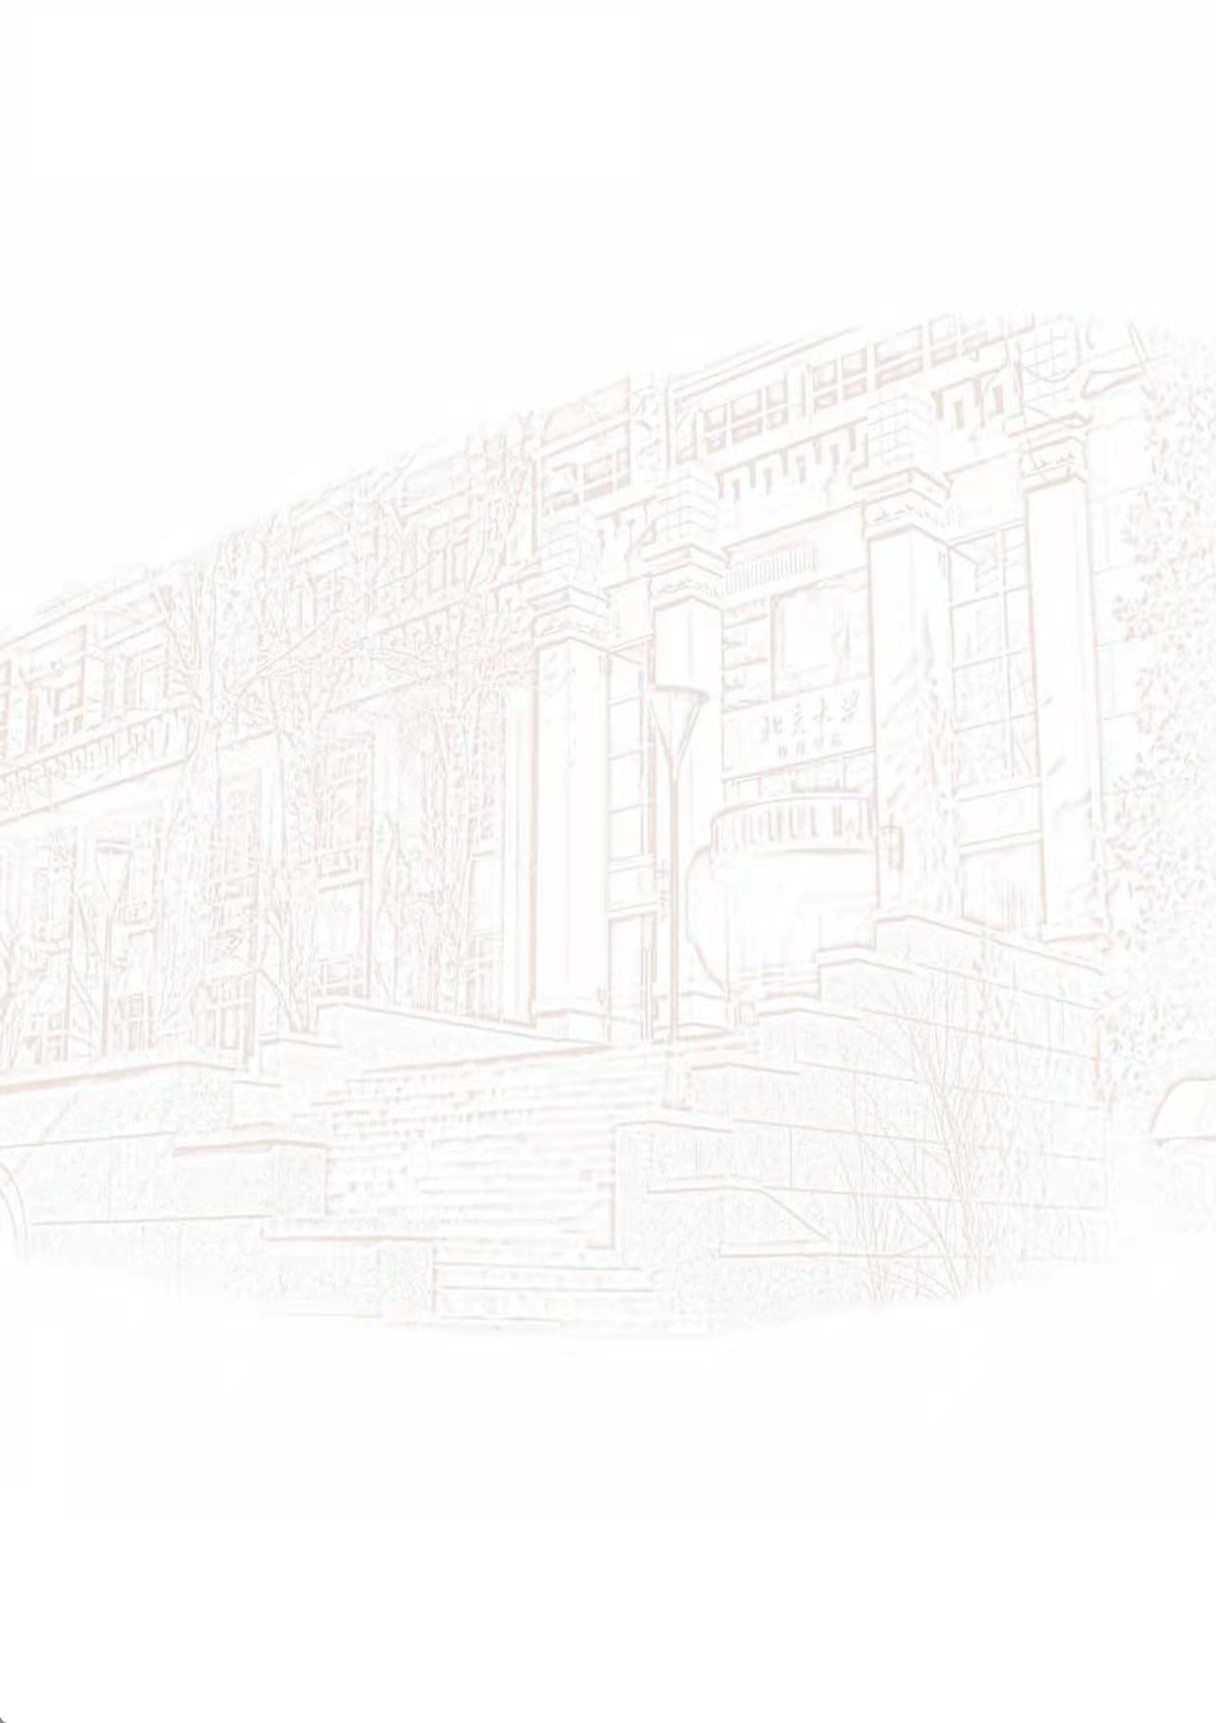
\includegraphics[width=\paperwidth, height=\paperwidth, keepaspectratio]{pic/phy.jpg}}}
%\ctexset{punct=kaiming}
\setCJKmainfont[ItalicFont=FZKTK.TTF,BoldFont=FZXBSK.TTF]{FZSSK.TTF}
\setCJKsansfont[BoldFont=FZHTK.TTF]{FZXH1K.TTF}
\setCJKmonofont[ItalicFont=FZKTK.TTF]{FZFSK.TTF}
\newCJKfontfamily\FZSS{FZSSK.TTF}
\newCJKfontfamily\FZKT{FZKTK.TTF}
\newCJKfontfamily\FZFS{FZFSK.TTF}
\newCJKfontfamily\FZHT{FZHTK.TTF}
\setmainfont{TeX Gyre Termes}
\setsansfont{TeX Gyre Heros}[Scale=MatchLowercase]
\setmonofont{Ubuntu Mono}%[Scale=MatchLowercase]
\newfontfamily\lm{Latin Modern Roman}
\usepackage{unicode-math}
\setmathfont{TeX Gyre Termes Math}
\usepackage{abstract}
\setlength{\absleftindent}{0pt}
\setlength{\absrightindent}{0pt}
\newcommand\keywords[1]{\textbf{Keywords}: #1}
\newcommand\pkg[1]{\textsf{#1}}
\newenvironment{csop}{\vskip\topsep\noindent\hspace{2em}\ttfamily\small\ignorespaces}{\vskip\topsep\par}
\usepackage{float}
\usepackage{booktabs,metalogo,siunitx,marginnote,manfnt,url}
\usepackage[unicode]{hyperref}
\hypersetup{pdfstartview=XYZ,hidelinks,pdfcreator=XeTeX Output,pdfauthor=Wu Xinan,
pdftitle=phyasgn文档类}
\usepackage{geometry,fancyhdr}
\geometry{left=3cm,right=3cm,marginparwidth=4em}
\fancyhead[L]
{\begin{tabular}[b]{@{}l@{}}
  \hyperref{https://www.pku.edu.cn/}{}{}{
\includegraphics[height=2.3em]{pic/pkulogo.jpg}}
\end{tabular}}
\fancyhead[C]
{\begin{tabular}[b]{@{}c@{}}
  \large
  Carbon Nanotubes for Ultrafast Photonics
  \\[-2pt]
  {\scriptsize Name:~Wu Xinan\quad ID:~1900011413}
\end{tabular}
}

\usepackage{shortvrb,fancyvrb}
\MakeShortVerb|
\fvset{xleftmargin=2em,fontsize=\small}
\makeatletter
\ifx\l@nohyphenation\undefined
  \newlanguage\l@nohyphenation
\fi
\DeclareRobustCommand\meta[1]{%
  \ensuremath\langle
  \ifmmode \expandafter \nfss@text \fi
  {%
    \rmfamily\itshape
    \edef\meta@hyphen@restore
    {\hyphenchar\the\font\the\hyphenchar\font}%
  \hyphenchar\font\m@ne
  \language\l@nohyphenation
  #1\/%
  \meta@hyphen@restore
  }\ensuremath\rangle
}
\makeatother

\def\phyasgn{\pkg{phyasgn}}
\def\version{0.2 $\upbeta$}

\title{
  {Carbon Nanotubes for Ultrafast Photonics}\\[-8pt]
  {\normalsize ——Ultrafast Laser and Spectroscopy Final Report}
}
\author{Wu Xinan}
\date{}

\begin{document}
\maketitle

\begin{abstract}
\vspace{-1.3em}
 Carbon nanotubes (CNTs) possess both remarkable optical properties and high potential for integration in various photonic devices. For example, nanotube-based saturable absorbers(SAs) can be used as all-optical switches, optical amplifier noise suppressors, or mode-lockers to generate ultrashort laser pulses. In this article, we discuss fundamentals and fabrication of CNTs, mode-locked fiber lasers using CNT-based SA and their applications in frequency combs.
\end{abstract}
\keywords{Carbon nanotube, Saturable absorber, Mode-locked fiber lasers, Frequency comb}
\tableofcontents

\section{Introduction}
Material science plays an important role in the current development of photonics providing new nonlinear materials, low loss transparent or opaque media, and creating new applications, optical technologies and devices, especially nonlinear optical materials. Optical nonlinearity is exploited in various photonic applications, such as, switching, routing and regeneration of optical signals, as well as for generation of ultrashort laser pulses\cite{10.1049/ip-j.1992.0001}.  
\par However, for ultrafast applications, nonlinear optical materials must possess a high nonlinear susceptibility and a fast recovery time. Single Wall Carbon Nanotubes (SWNTs) are of great interest in photonics and optoelectronics due to their non-linear optical properties and a fast recovery time. Features in the optical absorption and emission spectra are generated by excitonic transitions\cite{wang2005optical}. SWNTs show strong third order nonlinearities through these excitonic transitions, as they become more transparent when irradiated by high power (saturable absorption, SA)\cite{chen2002ultrafast,tatsuura2003semiconductor}. SWNTs are thus suitable for application as saturable absorbers in passively mode-locked lasers\cite{sakakibara2005carbon}. SWNTs are also a promising candidate for the ultrashort pulse generation because they possess ultrafast excited state carrier dynamic and high optical nonlinearity. In 2003, SWNTs were applied in fiber laser for passive mode-locking for the first time\cite{chen2002ultrafast}. 
\par There are numerous reports in the literature\cite{goh2005femtosecond,wang2008f,kelleher2010bismuth,solodyankin2008mode,kieu2008all,kelleher2009nanosecond,fedotov2012spectrum,liu2008passively,yu201366,ismail2012nanosecond,liu2015distributed,dong2011short,noronen2015all,ahmad2014mode,chernysheva2014sesam,chernysheva2014higher} on the use of SWNTs as mode-lockers and Q-switches for ultrafast lasers. One of the main advantages of SWNT-based SA except the short recovery time and high nonlinearity, is the ease of their fabrication and implementation into the laser setup. 
\par In Section 2 of this paper, we will introduce some fundamentals of CNTs, including their electrical and linear optical properties and their properties of saturable absorption. After that, in Section 3, we will describe the synthesis of CNTs. There are four methods in this part(arc discharge method, laser ablation, CVD method and CoMoCAT method). In Section 4, we will introduce short pulse fiber lasers with CNT-based SA. According to the different doping materials, we divide the short pulse fiber lasers into four types, and introduce their characteristics and research progress respectively. Then, in Section 5, we will describe an important role of mode-locked fiber lasers, the generation of coherent broadband spectra (frequency combs) through supercontinuum (SC) processes in highly nonlinear fibers (HNLFs). Finally, we make a conclusion of the content above.
\section{Fundamentals of CNTs}
\subsection{Electrical and linear optical properties}
CNTs can be classified into Multi Wall and Single Wall Nanotubes (MWNTs and SWNTs). A SWNT is a rolled tubule of single-layer graphene with end-caps; So it can be considered as a long 1D material. The CNT structure is determined by how the single-layer graphene is folded; the characteristic is expressed by a single parameter, and its chirality is expressed by a chiral vector \textbf{C$_h$} = (n, m) with two integers n and m that specifies the connecting points in folding of the 2D graphene(\figref{2}). 
\begin{figure}[!h]
	\centering
	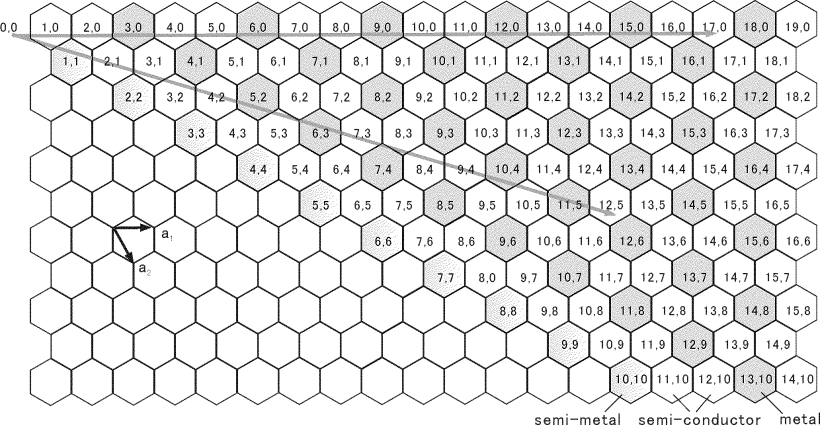
\includegraphics[width=.85\linewidth]{pic/2.png}
	\caption[Chiral vector (n,m) representation on a 2D graphene]{Chiral vector (n,m) representation on a 2D graphene\cite{set2004ultrafast}}
	\label{2}
	\end{figure}
\par When a 2D graphene is folded to a 1D CNT, there will be an additional quantization arising from electron confinement around the CNT circumference. The periodic
boundary condition is \textbf{C$_h$}$\cdot \kappa$ = 2q$\pi$ (where q is an integer). As a result, the electronic band structure of a specific CNT is given by the superposition of the cuts of the graphene electronic energy bands along the corresponding allowed $\kappa$ lines. When one of these cuts contains the Dirac (K) point, the CNT is metallic (metallic CNT: m-CNT, \figref{1}). Otherwise, it will become semiconducting (semiconducting CNT: s-CNT, \figref{1}). It is easy to know that n − m = 3k (where k is an integer) is suitable for m-CNTs, and n − m $\neq$ 3k is for the s-CNTs (\figref{2}, chiral vectors in white cells are semiconductor, while those in grey cells and semigrey cells are metallic and semimetallic). 
\begin{figure}[!h]
	\centering
	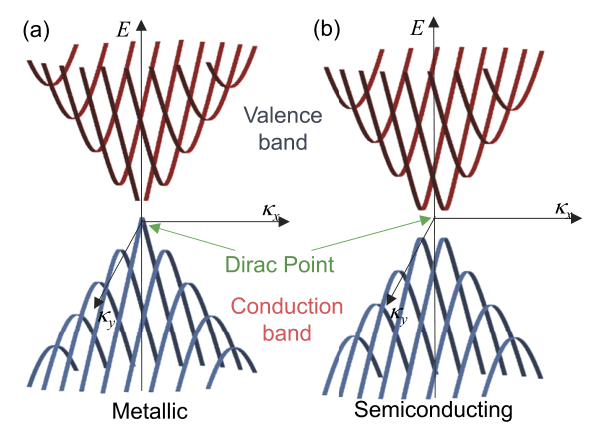
\includegraphics[width=.65\linewidth]{pic/1.png}
	\caption[Band structures]{Band structures of different types of nanotubes\cite{set2004ultrafast}}
	\label{1}
	\end{figure}
\par For a CNT, optical transitions can occur between the bandgaps v$_1$–c$_1$, v$_2$–c$_2$, . . ., the bandgap energy is inversely proportional to the tube diameter d. \figref{4} shows a typical transmission spectrum of a CNT sample. The S$_1$ and S$_2$ peaks correspond to the absorption between the bandgap transitions v$_1$–c$_1$ and v$_2$–c$_2$. The peak absorption wavelength $\lambda_p$ is proportional to the tube diameter d. So the absorption wavelength of a CNT sample can be engineered by choosing a proper tube diameter.
\begin{figure}[!h]
	\centering
	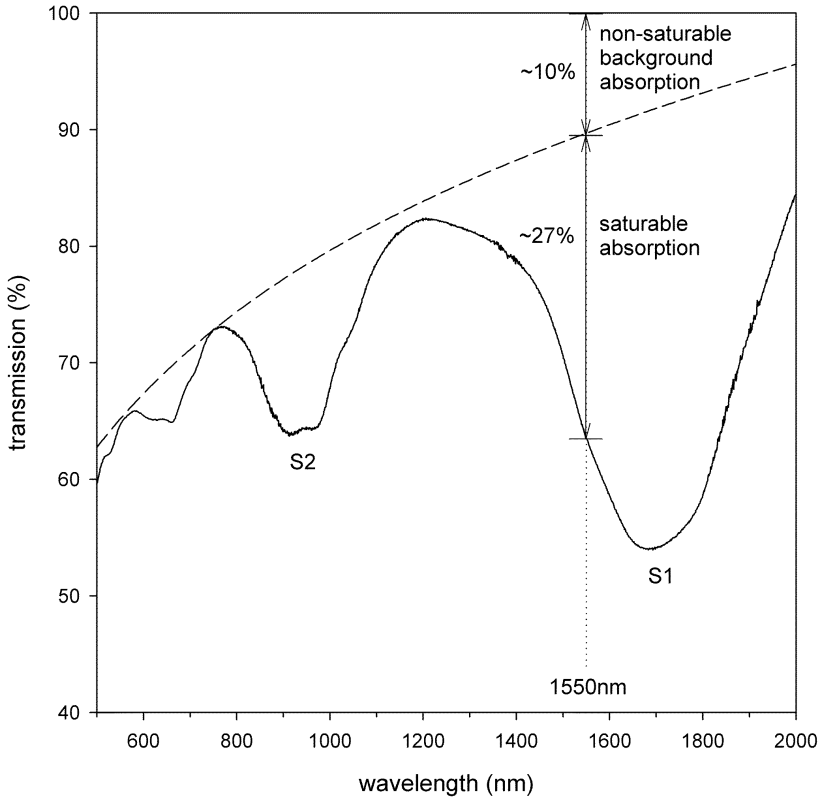
\includegraphics[width=.6\linewidth]{pic/4.png}
	\caption[Band structures]{Transmission spectrum of SAINT (solid line) showing the saturable absorption and the nonsaturable loss (dashed line)\cite{set2004ultrafast}}
	\label{4}
	\end{figure}
\subsection{Saturable absorption(SA)}
In general, assuming an instantaneous dielectric response in an isotropic material, the relation between an induced polarization [P(t)] and an electric field [E(t)] is expressed by:
\begin{equation}
P(t)=\varepsilon_0(\chi^{(1)}E(t)+\chi^{(2)}E^{2}(t)+\chi^{(3)}E^{3}(t)+\cdots )
\end{equation}
where $\varepsilon_0$ is the permittivity of a vacuum, $\chi^{(1)}$ is the linear susceptibility, and $\chi^{(2)}$ and $\chi^{(3)}$ are the second and third-order nonlinear susceptibilities.
\par The second-order nonlinearity $\chi^{(2)}$ is nonzero only for the material that lacks an inversion symmetry at the molecular level. Since the honeycomb carbon structure has the inversion symmetry, both CNT and graphene do not possess the second-order nonlinearity, unless the symmetry is disturbed. $\chi^{(2)}$ is related to the electro-optic effect, such as the Pockels effect.
\par The third-order nonlinearity $\chi^{(3)}$ is responsible for nonlinear Kerr effect, saturable absorption and multi-photon absorption. The $\chi^{(3)}$ nonlinearity has been shown to be very large in CNTs. The optical absorption are dependent on the incident optical intensity, and the complex refractive index n can be expressed as:
\begin{equation}
n=n_0+n_2I-i\dfrac{\lambda}{4\pi}(\alpha_0+\alpha_2I)
\end{equation}
where I is the optical intensity, n$_2$ is the nonlinear refractive index, and $\alpha_2$ is the nonlinear absorption coefficient. Both n$_2$ and $\alpha_2$ are interrelated with the real and complex part of $\chi^{(3)}$:
\begin{equation}
n_2=\dfrac{3}{4n_0^2\varepsilon_0c}Re(\chi^{(3)}),\quad \alpha_2=\dfrac{-3\omega}{2n_0^2\varepsilon_0c^2}Im(\chi^{(3)})
\end{equation}
\par Saturable absorption (SA) is a phenomenon related to the imaginary part of $\chi^{(3)}$ like the equation above, where high intensity light bleaches the material and reduces the optical absorption, it can be expressed as:
\begin{equation}
\alpha=\dfrac{\alpha_0}{1+I/I_S}
\end{equation}
where $\alpha_0$ is the linear absorption coefficient and I$_S$ is the saturation intensity.
\par CNTs have ultrafast saturable absorption responses\cite{chen2002ultrafast,tatsuura2003semiconductor}. \figref{9} depicte the optical absorption of CNTs. Saturation takes place when all the allowed states in the conduction band are fully populated and the valence band emptied at high optical intensities(\figref{9}).
\begin{figure}[!h]
	\centering
	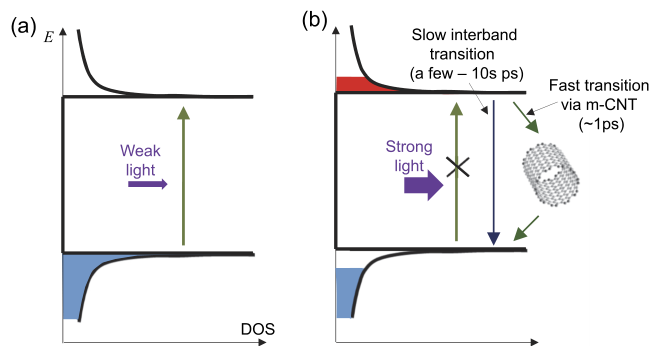
\includegraphics[width=.7\linewidth]{pic/9.png}
	\caption[Band structures]{Optical absorption and saturation in CNTs\cite{martinez2013nanotube}}
	\label{9}
	\end{figure}
\par S-CNTs are good SA materials due to their ultrafast recovery time and high third order nonlinearity. However, there will be high losses due to residual large aggregates as well as catalyst particles or the formation of bubbles when SWNTs were used in suspension\cite{yamashita2004saturable}. The best way to overcome such disadvantages is to finely disperse SWNTs in a polymer matrix\cite{yamashita2004saturable}.
\par Before choosing a suitable polymer matrix for the preparation of a nonlinear optical device with SWNTs, we need to consider that SWNTs is a special material with chirality dependent electronic structures, and SWNTs are the strongly hydrophobic material with strong van der Waals attraction between tubes. So it is difficult to disperse raw SWNTs directly into the polymer matrix without covalent fictionalisation.
\par Nowadays, SWNT-water soluble polymers (mostly PVA) saturable absorbers have dominated. The reason is that the control of the concentration of SWNTs and SWNT bundle size is easy. And the thickness of composite allows engineering of a saturable absorber with specific recovery time, modulation depth, saturation intensity and nonsaturable loss.
\section{CNT synthesis}
The first SWNTs were synthesized using the arc discharge method\cite{kundrapu2012model}, followed by the laser ablation method\cite{hutchens2012vertically}. But nowadays, most of the commercially available SWNTs are produced in a large scale by various chemical vapor deposition (CVD) methods\cite{li2004preferential,resasco2002scalable}.
\subsection{Arc discharge method}
The arc discharge method is the first established procedure for CNT production. It was initially developed for C$_{60}$ fullerenes and later transformed for MWNT\cite{charlier2001growth} and SWNT\cite{bethune1993cobalt} fabrication. Typically, the arc discharge method uses arc vaporisation of two carbon electrodes placed a small distance from each other, about 1–2 mm in a cavity filled with inert gas at low pressure or liquids(\figref{5}). The medium ionisation results in plasma formation between the electrodes. The high temperature of anode sublimates carbon and evaporates it. The carbon vapours are disintegrated in carbon ions due to thermal energy in plasma. The carbon gases move along the temperature gradient towards the relatively cool cathode, condense into liquid carbon and later crystallises, forming rod-shaped deposition on the cathode, which is composed of CNTs\cite{arora2014arc}. 
\begin{figure}[!h]
	\centering
	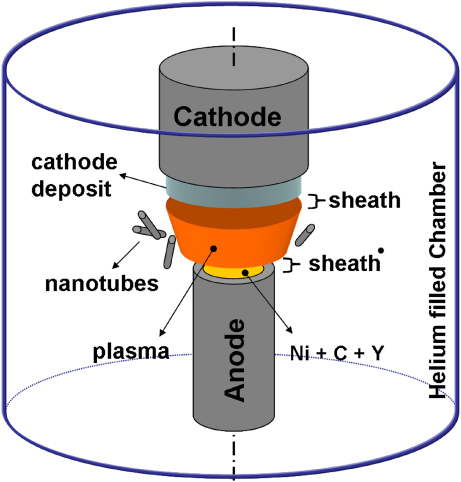
\includegraphics[width=.5\linewidth]{pic/5.jpg}
	\caption[Band structures]{Schematic of a carbon arc discharge for the synthesis of nanoparticles\cite{kundrapu2012model}}
	\label{5}
	\end{figure}
\par One of factors affecting CNT growth is catalysts. It was experimentally shown that the presence of metal catalyst favours SWNT growth, rather than MWNTs, whereas the size of the catalyst determines the diameter distribution\cite{lin1994large}. Moreover, the pressure of inert gas determines the structure of the carbon product. Under different pressure conditions, different products such as carbon onions, nanotubes, fullerene and amorphous graphite may appear\cite{wilson2002nanotechnology}.
\par In conclusion, the arc discharge method is one of simplest ways, allowing low-cost production of CNTs, and it has advantages of rapid production with fewer topological defects\cite{kundrapu2012model}.
\subsection{Laser ablation}
Not long after laser was invented, the laser ablation process uses a pulsed laser to hit a graphite target\cite{hutchens2012vertically}. An inert gas carries carbon vapours along the tem-perature gradient from the high temperature into a cooled collector positioned downstream (\figref{7}). Out of evaporated graphite, carbon nanotubes are formed and deposited on the chamber wall. Produced nanotubes are bundled, aligned along a common axis and form a mat of ropes. The yield of SWNTs out of the carbon consumed by laser ablation is more than 70\%\cite{thess1996crystalline}. 
\begin{figure}[!h]
	\centering
	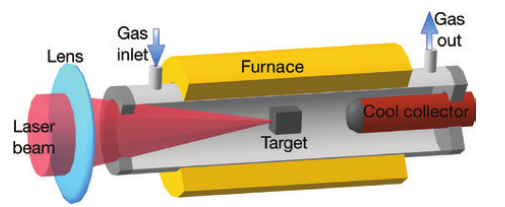
\includegraphics[width=.85\linewidth]{pic/7.png}
	\caption[Band structures]{Schematic of a laser ablation for the synthesis of nanoparticles\cite{hutchens2012vertically}}
	\label{7}
	\end{figure}
\par Analogous to the arc discharge method, laser ablation also utilises catalysts to grow tubes on their atoms\cite{yudasaka1997single}. Catalysts are essential in nanotube formation as their atoms prevent the closing of the fullerene by attaching additional carbon particles. A single atom or group of atoms adsorb carbon molecules transforming them into rolled graphene-like sheets until too many catalyst atoms accumulate at the end of the nanotube\cite{guo1995catalytic}.
\par Overall, similar to the arc discharge method, laser ablation method produces small quantities of high-quality CNTs, but does not have the capacity for large-scale production. And SWNTs grown by the laser ablation method usually have a narrow diameter and can be applied for Er, Tm and Ho-doped fiber lasers. 
\subsection{Chemical vapour deposition(CVD)}
The chemical vapour deposition (CVD) method is the most promising technique for the large-scale production of CNTs. CVD nanotubes feature a small diameter distribution in the range from 1 to 3 nm and high aspect ratios of more than 10$^4$. Moreover, such SWNTs benefit from smooth curving and the small amount of topological defects along sidewalls.
\par During the CVD process, the patterned substrate is heated in the chamber filled with inert gas (\figref{6}). The gas of carbon feedstock flows into the chamber to replace the inert gas until the furnace cools to room temperature. The growing process of nanotubes includes absorption, decomposition of carbon feedstock on catalytic particles and diffusion of carbon particles into catalysts from a supersaturated catalyst surface. 
\begin{figure}[!h]
	\centering
	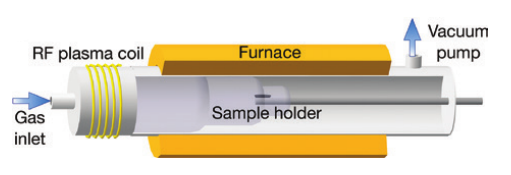
\includegraphics[width=.85\linewidth]{pic/6.png}
	\caption[Band structures]{Schematic of a CVD method for the synthesis of nanoparticles\cite{li2004preferential}}
	\label{6}
	\end{figure}
\par The “base-growth” is the dominating mechanism for SWNT materials. The CVD method utilises a mixture of hydrocarbon gas and process gas (nitrogen, hydrogen or ammonia), which react in a chamber on a substrate, heated to the temperature of 700–900 $^{\circ}C$. A substrate is covered with catalytic metal particles, like Fe, Ni, Co or their combination. Patterning the substrate with catalysts allows SWNT growth at a particular position. And similar to previously discussed methods, catalysts play a critical role in the CVD process, determining the yield and type of final carbon  products\cite{cassell1999large}.
\par Although it will have small amount of topological defects along sidewalls using CVD method, the product can be scaled for mass production purposes. Consequently, chemical methods are considered to be more promising.
\subsection{Cobalt and molybdenum (CoMo) CAT process}
CoMoCAT process is a new method to grow SWNTs, it can produce about 0.25 g SWNT/g catalyst in a couple of hours and the amount of SWNT could reach 80\%\cite{kitiyanan2000controlled}.
\par This method is based on the CO decomposition described by the Boudouard reaction:
\begin{equation}
CO+CO=C(s)+CO_2(g)
\end{equation}
\par The temperature of the CO gas usually ranges between 700$^{\circ}$C and 950$^{\circ}$C with the pressure from 1 to 10 atm. After the reaction of CO disproportionation begins, Mo oxide transforms into Mo carbide. Metallic Co particles being dispersed in the chamber hit CO molecules. CO molecules decompose and nucleate until a certain configuration and carbon surface concentration are obtained for CNT formation (\figref{8}). The configuration of this embryo determines the diameter of the future nanotube. The following formation of CNTs by incorporation of carbon onto the embryo only takes several milliseconds. With the temperature growth, larger metal clusters are formed on the catalyst surface, which cause the production of nanotubes with larger diameters\cite{resasco2002scalable}.
\begin{figure}[!h]
	\centering
	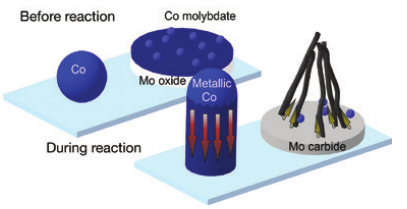
\includegraphics[width=.85\linewidth]{pic/8.png}
	\caption[Band structures]{Schematic of a CoMoCAT method for the synthesis of nanoparticles\cite{resasco2002scalable}}
	\label{8}
	\end{figure}
\par The presence of two simultaneous catalysts Co and Mo is essential for CNT formation. Temperature also plays a critical role in all of these processes, determining their efficiency and yield. 
\par In fact, CoMoCaT SWNTs of small diameters (0.7-1.1 nm) perfectly works in Yb and Bi-doped fiber lasers. And it was widely used in industry nowadays. 
\section{Mode-locked fiber lasers with CNT-based SA}
By including a proper saturable absorber (SA) in a laser cavity, an ultra-short optical pulse train can be generated through passive mode-locking\cite{keller2003recent}, as illustrated in \figref{10}. 
\begin{figure}[!h]
	\centering
	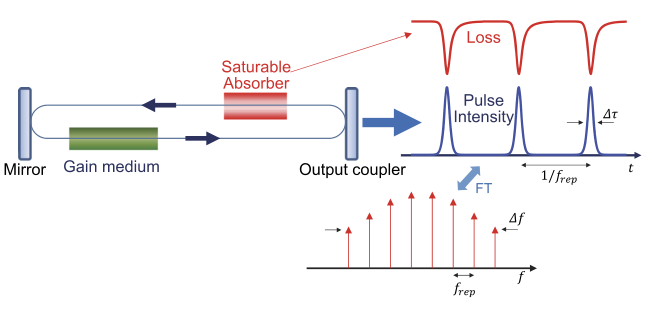
\includegraphics[width=.9\linewidth]{pic/10.png}
	\caption[Band structures]{Passively mode-locked laser using the saturable
    absorber\cite{keller2003recent}}
	\label{10}
	\end{figure}
\par It first starts from the spontaneous emission noise of the gain medium of the laser. When a SA is placed in the laser cavity, the large components of the spontaneous emission noise tend to survive through the SA, these components are then amplified by the gain medium by the SA. Thus, this process is iterated repeatedly to form a stable pulse train so that a single or an integer number of pulses circulate in the laser cavity. In fundamental mode-locking, which is crucial for a stable operation, the repetition frequency ($f_{rep}$) is equal to the free spectral range (FSR) of the laser cavity. It can be expressed as:
\begin{equation}
f_{rep}=\dfrac{c}{nL}
\end{equation}
where L is the laser cavity length and n is the index of the laser cavity. 
\par It should be noted that CNTs need to be incorporated in an optical fiber or waveguide systems so that they can interact with light efficiently. One way is to develop the interaction of the evanescent field of the light propagating in the fiber with CNT-based SA. The nonlinear materials interact with the evanescent field, whilst the interaction length is extended profoundly to achieve a large amount of nonlinear effects. Here are three examples of fiber-type CNT/2D-SA devices in \figref{11} with evanescent field interaction.
\begin{figure}[!h]
	\centering
	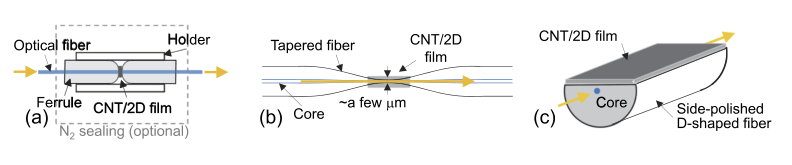
\includegraphics[width=1.0\linewidth]{pic/11.png}
	\caption[Band structures]{Fiber-type CNT/2D-SA devices\cite{song2007polarization}}
	\label{11}
	\end{figure}
\par Nowadays, fiber lasers are the most commonly mode-locked with SWNTs, due to the ease of coupling SWNT–composites into a fiber laser. In addition, they normally require large modulation depths in order to stabilize the intracavity pulses, which can be provided by the relatively large nonlinearity of the SWNT mode-lockers. The spectral coverage of SWNT-enabled fiber lasers is superior to that of conventional SESAMs, especially for over 1.3 $\mu$m spectral range. We can also select the SWNT SAs operating band by varying the mean tube diameter. In fact, SWNT-based SAs have successfully mode-locked Yb-doped\cite{goh2005femtosecond}, Er-doped\cite{wang2008f}, Bi-doped\cite{kelleher2010bismuth} and Tm-doped\cite{solodyankin2008mode} fiber lasers.
\subsection{Yb-doped fiber lasers}
Mode-locked operation of a Yb-doped fiber laser with CNT-based SA was first demonstrated in 2005\cite{goh2005femtosecond}. The Yb-doped fiber laser produced 180 fs long solitons at a repetition rate of 23.3 MHz. This laser had a transmissiontype SA incorporating CNTs with saturable absorption depth of 4\%. Then in 2008, the possibility of mode-locking in a Yb-doped fiber laser with CNT in an all-fiber configuration with a tapered fiber embedded in a composite CNT-polymer was demonstrated\cite{kieu2008all}. The normal dispersion laser cavity provided generation of 1.5 ps chirped pulses, which could be compressed down to 250 fs outside the cavity\cite{kieu2008all}. And in 2009, the pulse duration could adjust between 21 MHz and 177 kHz within the range from 20 ps to 2 ns at repetition rates\cite{kelleher2009nanosecond}. 
\par \figref{12} shows the schematic diagram of the Yb ring laser with a Lyot filter. The SA was represented by a polymer film with prepared CoMoCATs SWNT. Utilisation of a fiber Lyot filter enables the variation of the laser output spectrum width within the 0.15–1.25 nm range and detuning the central wavelength by up to 5 nm\cite{fedotov2012spectrum}.
\begin{figure}[!h]
	\centering
	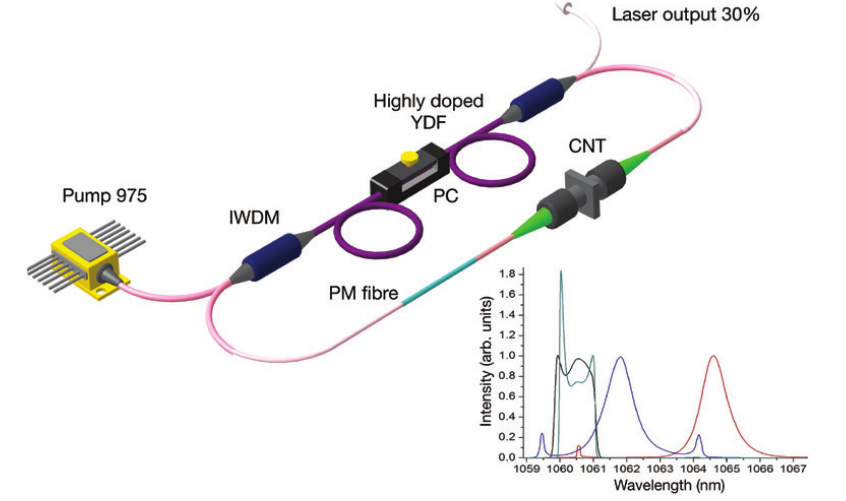
\includegraphics[width=.95\linewidth]{pic/12.png}
	\caption[Band structures]{Schematic of Yb-doped fiber laser setup, Inset: Central wavelength tuning\cite{fedotov2012spectrum}}
	\label{12}
	\end{figure}
\par CNT-based SA may be used in Yb-doped fiber lasers both for mode-locking and for Q-switching, and CNTs may be used in fiber lasers not only as mode-lockers but also as polarisation controllers, owing to anisotropic properties of CNTs.
\subsection{Er-doped fiber lasers}
In 2008, both linear and ring Er-doped fiber lasers were studied\cite{liu2008passively}, and up to now, CNT mode-locked Er-doped fiber lasers have been widely studied. The shortest pulse duration generated, in CNT mode-locked Er-doped fiber lasers is 66 fs long\cite{yu201366}, while the longest one is 332 ns long\cite{ismail2012nanosecond}. The broad bandwidth of CNT allows spectral tuning in the range from 1532-1562 nm and multiwavelength generation\cite{liu2015distributed}.
\par CNT mode-locked Er-doped fiber lasers exhibit harmonic mode-locking by sustaining stable operation at the 10th or even 23rd harmonic of the repetition frequency\cite{liu2008passively}. The laser setup presented in \figref{13} constitutes 80 cm of highly doped erbium fiber, the PVA/ SWNT-based SA sandwiched between fiber ferrules. The laser supported 10th harmonic at a pump power of 141 mW showing a repetition rate of 245 MHz\cite{liu2008passively}. 
\begin{figure}[!h]
	\centering
	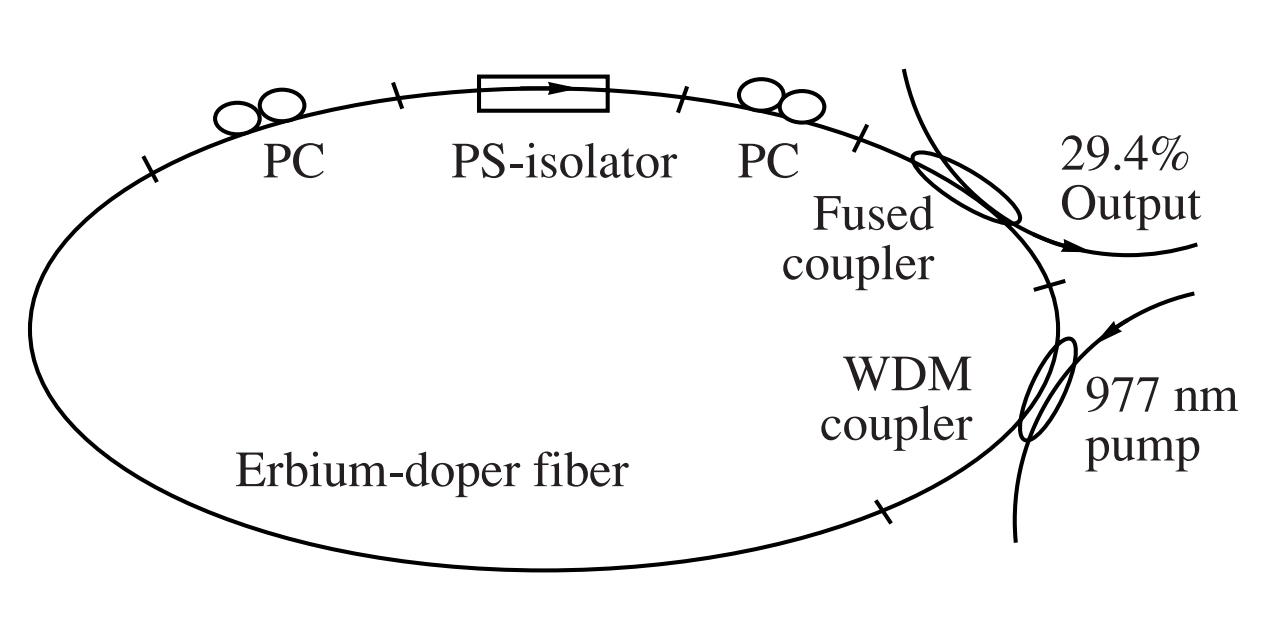
\includegraphics[width=.9\linewidth]{pic/13.png}
	\caption[Band structures]{Schematic of Er-doped fiber laser setup\cite{liu2008passively}}
	\label{13}
	\end{figure}
\par Er-doped fiber lasers with CNT can also be passively Q-switched, providing a comparatively high level of output pulse energy at shorter pulse durations of 662 ns\cite{dong2011short}.
\subsection{Bi-doped fiber lasers}
To adapt various applications in broadband data transmission, medical applications and for high-brightness frequency-doubled visible sources have drawn the research interest to the extension of fiber laser emission band to 1100–1550 nm. In contrast with rare earth-doped active fibers, which cannot provide generation at this band, Bi-doped fibers have shown the broad gain in the region, favourable for ultrashort pulse formation. 
\par The first Bi-doped fiber laser to produce ultrashort pulses by using the SWNT-based SA was proposed and realised in 2010\cite{kelleher2010bismuth}. The generation was achieved in both All-Normal Dispersion (ANDi) and Dispersion-Managed (DM) net anomalous cavity at 1157 and 1177 nm band. The ANDi laser generated 558 ps pulses having the energy of 1.4 nJ, whereas the DM cavity operated in the average-soliton regime with a 4.7 ps duration and the energy of about 3 pJ.
\begin{figure}[!h]
	\centering
	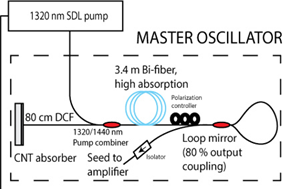
\includegraphics[width=.75\linewidth]{pic/14.png}
	\caption[Band structures]{Schematic of Bi-doped fiber laser setup(MOPA)\cite{noronen2015all}}
	\label{14}
	\end{figure}
\par However, the most recent work now is focused on the development of a 1.44 $\mu$m All-Bismuth fiber Master Oscillator-Power Amplifier (MOPA) system in \figref{14}. Scientists used butt-coupled SWNT-based SA deposited onto a silver mirror to support the mode-locked operation. After amplification and compression, the laser generates 240 fs pulses with 3.1 kW peak power\cite{noronen2015all}.
\par Further works aimed to broaden the generation to the telecommunication L-band. For this, Bi-Er co-doped optical fibers were used as an active gain\cite{ahmad2014mode}. 
\subsection{Tm-doped fiber lasers}
The increasing demand for low-cost highly stable ultrafast laser generation at the mid-IR spectral region (about 2 $\mu$m), has stimulated a significant research of the development of the Tm-doped fiber lasers. 
\par In 2008, scientists first introduced this technique to Tm-doped fiber lasers\cite{solodyankin2008mode} (the schematic is in \figref{15}). The NALM is formed by a 20:80 fiber coupler and normal dispersion germanium-silica fiber (GeO$_2$/SiO$_2$). A polymer film based on carboxymethylcellulose (CMC) with dispersed arc discharge SWNTs is fixed between two angle-polished optical ferrules. The shortest pulse duration of 450 fs at 1870 nm central wavelength band has been achieved when the total was zero NALM dispersion. The maximum average output power could be scaled from 6.3 to 18 mW , corresponding to the laser peak power of 625 W and pulse energy of 0.4 nJ.
\begin{figure}[!h]
	\centering
	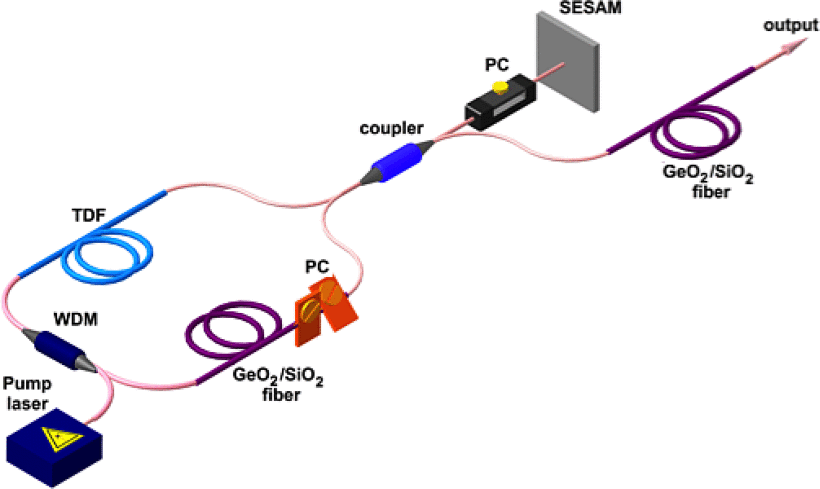
\includegraphics[width=.85\linewidth]{pic/15.png}
	\caption[Band structures]{Schematic of SESAM mode-locked Tm-doped fiber laser\cite{chernysheva2014sesam}}
	\label{15}
	\end{figure}
\par The development of high-power lasers without application of the complicated MOPA schemes is very attractive. Chernysheva\cite{chernysheva2014higher} present the high-power thulium-doped fiber ring laser with the variable pulse repetition rate between 6.4 and 72.5 MHz and tuneable from 1.86 to 1.98 $\mu$m\cite{chernysheva2014higher}. And it has the excellent long-term stability of the laser operation at 300 mW output power for 10 hours under the laboratory conditions. The laser setup with the cavity length of 21 m after compression generates 500 fs pulses with the average output power of 117 mW, corresponding to the pulse energy of 10.87 nJ and peak power of 21.7 kW\cite{chernysheva2014higher}.
\section{Applications}
Mode-locked fiber lasers using CNT-based SA have been applied as a short pulse source for a non-synchronous optical sampling scope and a label-free multi-photon microscopy. An important application of mode-locked fiber lasers is the generation of coherent broadband spectra (frequency combs) through supercontinuum (SC) processes in highly nonlinear fibers (HNLFs). 
\par A typical fiber-based SC source is depicted in \figref{16}. Short pulses are amplified by fiber amplifier, and then launched into a length of HNLF to broaden the spectrum through the nonlinearity in the HNLF. The octave spanning SC spectrum from 1 $\mu$m to over 2 $\mu$m has been generated using a CNT-based mode-locked fiber laser. The laser generates 220 fs pulses, and the pulses are amplified and compressed to 65 fs\cite{kieu2010generation}. The SC spectrum spans from 1 $\mu$m to more than 2 $\mu$m, as shown in \figref{16}. 
\begin{figure}[!h]
	\centering
	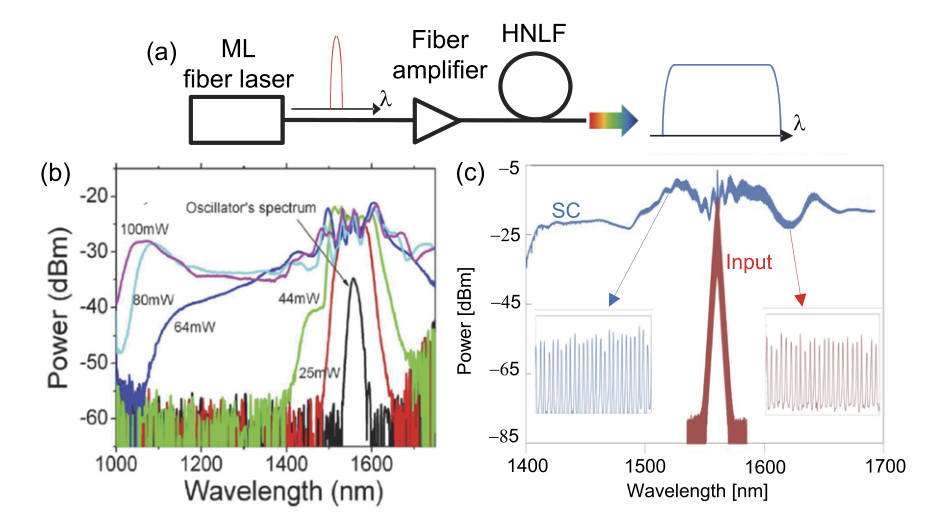
\includegraphics[width=.9\linewidth]{pic/16.png}
	\caption[Band structures]{Broadband frequency comb generation through SC in HNLF\cite{kieu2010generation}}
	\label{16}
	\end{figure}
\par Such broadband SC has been used, not only for laser stabilization using the f and 2f components but also for generating fs pulses at the 1 $\mu$m wavelength region, mid-IR frequency comb through difference frequency generation, synchronized ps pulses at 1 $\mu$m and 1.5 $\mu$m for Stimulated Raman Scattering (SRS) microscopy\cite{freudiger2014stimulated,tsuzuki2016midinfrared,kieu2010generation}.
\par In \figref{16}, it also depicts the SC spectrum generated by the aforementioned 1 cm long 10 GHz mode-locked FP laser using a CNT-based SA. We could obtain a flat SC spectrum spanning from 1.4 $\mu$m to over 1.7 $\mu$m. The mode structures in the SC spectrum are visible in the inset of \figref{16}, showing that it is a coherent SC frequency comb. There is a strong demand for such a sparse frequency comb source especially in the metrology, spectroscopy, microscopy and imaging field.
\section{Conclusion}
In this article, we have reviewed the current state-of-the-art in CNT fabrication, technologies and ultrafast photonic applications. The important SWNT-polymer composite application is as SA in fiber lasers for ultrashort pulse generation through the passive mode-locking. 
\par CNT photonics has developed for about 20 years. Mode-locking using CNT-based SA is now a well-established technology, and is suitable for short pulse fiber lasers where the lasing wavelength matches with the absorption wavelength of CNTs. Moreover, other types of the lasers except fiber lasers, mode-locked by CNT-based SA, can potentially enable further technological enhancements. CNT-based photonics can develop new photonic techniques for various emerging applications, and lead to new breakthroughs in science and technology.
\appendix
\section{Acknowledgement}
Here I would like to thank Prof. Shi and Dr.Mu for your guidance throughout the semester, which has benefited me a lot. This is my first time to write a report in English. It took me a lot of time to look up materials and write, but I learned a lot from it, and at the same time, I have a better understanding of carbon nanotube research.
\par Before writing this article, I had taken courses in nonlinear optics, wide bandgap semiconductors, and introduction to nanoelectronic devices. This helped me a lot with my writing. I completed Section 2 with reference to the nonlinear optics course handout. And in the course of wide-bandgap semiconductors and nanoelectronic devices, I learned the general preparation method of carbon nanotubes, thus completing Section 3. Then, I went through the extensive material on carbon nanotubes for ultrafast photonics and finished the rest part. 
\par Hope this course will be better and more students will take this course next semester!
\printbibliography[heading=bibintoc]
\end{document}